%% Settings for single-side (simplex) printing
% Margins: left 40mm, right 25mm, top and bottom 25mm
% (but beware, LaTeX adds 1in implicitly)
\documentclass[12pt,a4paper]{report}
\setlength\textwidth{145mm}
\setlength\textheight{247mm}
\setlength\oddsidemargin{7.5mm}
\setlength\evensidemargin{7.5mm}
\setlength\topmargin{0mm}
\setlength\headsep{0mm}
\setlength\headheight{0mm}
% \openright makes the following text appear on a right-hand page
\let\openright=\clearpage

%% Character encoding: usually latin2, cp1250 or utf8:
\usepackage[utf8]{inputenc}

%% Prefer Latin Modern fonts
\usepackage{lmodern}

\usepackage{amsmath}        % extensions for typesetting of math
\usepackage{amsfonts}       % math fonts
\usepackage{amsthm}         % theorems, definitions, etc.
\usepackage{bbding}         % various symbols (squares, asterisks, scissors, ...)
\usepackage{bm}             % boldface symbols (\bm)
\usepackage{graphicx}       % embedding of pictures
\usepackage{fancyvrb}       % improved verbatim environment
\usepackage{natbib}         % citation style AUTHOR (YEAR), or AUTHOR [NUMBER]
\usepackage[nottoc]{tocbibind} % makes sure that bibliography and the lists
			    % of figures/tables are included in the table
			    % of contents
\usepackage{dcolumn}        % improved alignment of table columns
\usepackage{booktabs}       % improved horizontal lines in tables
\usepackage{paralist}       % improved enumerate and itemize
\usepackage[usnames]{xcolor}  % typesetting in color
\usepackage{float}
\usepackage[boxruled]{algorithm2e}
\usepackage{gensymb}

\usepackage{listings}
\usepackage{color}

\definecolor{dkgreen}{rgb}{0,0.6,0}
\definecolor{gray}{rgb}{0.5,0.5,0.5}
\definecolor{mauve}{rgb}{0.58,0,0.82}

\lstset{frame=tb,
  language=Java,
  aboveskip=3mm,
  belowskip=3mm,
  showstringspaces=false,
  columns=flexible,
  basicstyle={\small\ttfamily},
  numbers=none,
  numberstyle=\tiny\color{gray},
  keywordstyle=\color{blue},
  commentstyle=\color{dkgreen},
  stringstyle=\color{mauve},
  breaklines=true,
  breakatwhitespace=true,
  tabsize=3
}

\usepackage{enumitem}
\usepackage{courier}
\usepackage{epstopdf}
\begin{document}

% TITLE PAGE
\begin{titlepage}
    \begin{center}
        \vspace*{1cm}

        \Huge
        \textbf{Pepr3D}

        \LARGE

        \vspace{12cm}

		\Large
        \textbf{Authors}:
        Bc.~Štěpán Hojdar,
        Bc.~Tomáš Iser,
        Bc.~Jindřich Pikora,
		Bc.~Luis Sanchez
		\\
		\textbf{Supervisor}: Mgr.~Oskár Elek, Ph.D.
		\\
		\textbf{Consultants}: doc.~Ing.~Jaroslav Křivánek, Ph.D., Ing.~Vojtěch Bubník (Prusa Research~s.r.o.), Tobias~Rittig,~M.Sc.

        \vfill

		Faculty of Mathematics and Physics \\
		Charles University
    \end{center}
\end{titlepage}

%% TOC
\setcounter{tocdepth}{1}
\tableofcontents

% I. INTRO
\part{Introduction}

% Done for the most part
\chapter{Introduction}

In this project, we aim to create an intuitive application that allows the user to interactively color a 3D model and export it in a 3D printable format. This chapter will provide a brief summary of the 3D printing environment, its pipeline and the goals of the project which we set in the beginning.

\section{3D printing basics}

3D printing is a new technology that has seen rapid development in the last years. It comes in many different forms, melting plastic, fusing metals, shining UV on photopolymers, etc. Fused Deposition Modelling (FDM) is the most popular and accessible to the general public and for the purpose of this project, when we talk about 3D printing, we will always mean FDM printers, unless stated otherwise.

FDM printing is a relatively simple process - a printer head melts the plastic filament and deposits it on a preheated platform layer by layer, from the bottom towards the top. The printer has to regulate the temperature of both the filament in the head and the moving platform for the deposited material to bond correctly. Several types of filaments are used, namely PLA, ABS, PET and others.

\section{Prusa environment}

The Prusa environment is very similar to the general description we provided in the section 1.1. For the purpose of our project, the most important concept in the Prusa environment is the slicer. The slicer is a program that receives the 3D model the user wishes to print out and creates the instructions for the Prusa 3D Printer -- a G-code file. The file is then transferred to the printer, which then executes the commands in the G-code file. The slicer has to plan the movement of the head for the whole print. This includes several crucial things:

\begin{itemize}
\item Covering the whole area of each layer
\item Reinforcing the walls of the object to make them sturdier
\item Filling the inside of the object with a rougher print, because it won't be visible when finished
\item Planning the path so the head can stay in one Z level - an "Eulerian path".
\item Switching the materials for multimaterial printing (more in 1.3)
\end{itemize}

Prusa develop their own slicer - a forked branch of an open-source program called Slic3r \footnote{http://slic3r.org/}, called Slic3r Prusa Edition \footnote{https://www.prusa3d.com/slic3r-prusa-edition/}. This slicer can do all we listed above very well.

\section{Multimaterial printing}

Multimaterial printing is a very new concept, even in the fairly new world of 3D printing. Many of the simpler and cheaper 3D printers can only print one material models - one color for the whole object. However, many users would like to print models that include more than one color. Even though the more advanced printers are capable of combining up to four different materials into one print, the process to achieve this is rather cumbersome for the end user - the user has to manually split the 3D mesh of the object into parts that he wishes to have a different color.

For example, if we are printing a dragon, want the dragon to be black and have white teeth, we have to take the dragon model, and split off each individual tooth. Then tell the slicer that the remaining file - the toothless dragon should be black and the teeth should be white.

This model splitting has to be done in a full 3D editing software like Blender or 3ds Max, which is difficult to control for newcomers and overly complex.

\section{Our project}

Our project aims to make printing a multi-coloured object a lot easier, by developing an application that will allow the user to simply paint on the 3D model (i.e. the dragon) with different colors (i.e. color the teeth white), then simply click export and generate the files of the split-off models automatically.

Our application allows for free hand painting as well as some forms of guided painting -- bucket fill and some smarter tools, for example a bucket fill that studies the object's geometry and stops the filling if it detects a sharp edge (i.e. the transition of the tooth into the dragon).

The main goal is to make the application for desktop PCs, with main development time being focused on the Windows operating system. We did, however, use software engineering tools that can also be ported to a plethora of other platforms like Linux based OS, Mac OS and mobile, if the need should arise.


\chapter{Related work}

Based on our own research and the analysis of the experts from Prusa Research s.r.o, there, at the moment, does not exist a software that does what this project is trying to achieve. Here we present a simple list of software that could be used to achieve the same results as our program delivers. We highlight the pros and cons of each program to show that our goal is sufficiently unique.

\section{Autodesk Meshmixer}

The closest existing software is Autodesk Meshmixer \footnote{http://www.meshmixer.com/}, which is very complicated and is not targeted for FDM printing specifically. As such, it includes a lot of features that are not important for the FDM users and end up being confusing.

\section{Microsoft 3D Builder}

Microsoft 3D Builder \footnote{https://www.microsoft.com/en-us/p/3d-builder/9wzdncrfj3t6?activetab=pivot\%3Aoverviewtab} is another application that handles 3D models but we have not found a way to make it create anything remotely applicable to FDM printing.

\section{Complex 3D editors}

Any 3D computer graphics program designed to handle 3D models which allows for the model to be created or split by colors manually. This section would include software as 3ds Max, Maya or Cinema4D. Using these applications, however, would be very time comsuming for the user and practically unusable on a larger scale.



% II. DEVELOPER DOCU
\part{Developer Documentation}

% Should be similar to the Spec's corresponding chapter
\chapter{Architecture}

Now that we understand the background and use case of Pepr3D, we can propose a software architecture for the project.
In this chapter, we show an overview of the whole architecture.
Further details are then available in next chapters.

\section{Overview}

\begin{figure}[b]
	\centering
	\centerline{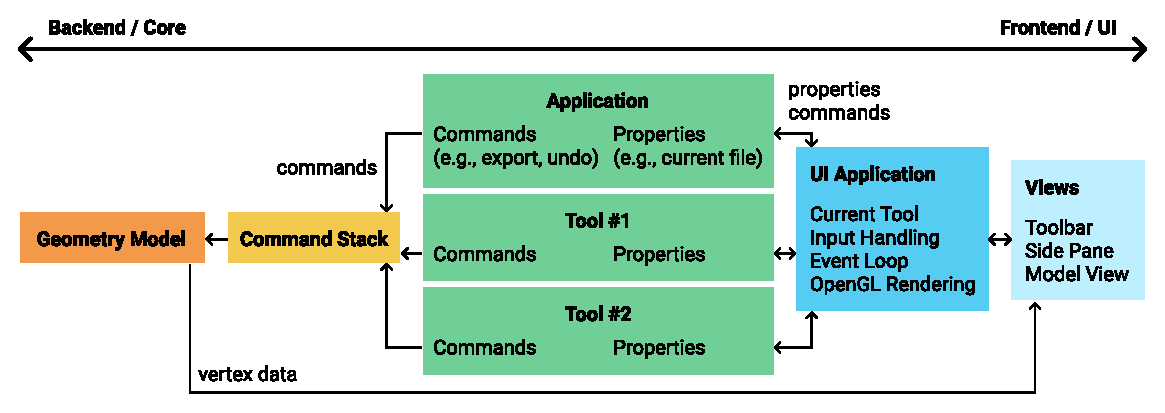
\includegraphics[scale=0.9]{images/architecture.eps}}
	\caption{An overview of the Pepr3D architecture.}
	\label{fig:architecture}
\end{figure}

A good software architecture should be easy to maintain and refactor, it should be possible to replace parts of it with new ones.
It should be as simple as possible, resistant to bugs and errors, and programs built with such architecture should run reasonably fast without any major bottlenecks.

This can be achieved with \emph{modularity}, i.e., separating a project into multiple parts that are as independent as possible.
It is important to define data flows and dependencies between the modules.
Keeping the data flows and dependencies as simple as possible makes it easy to replace modules in case it is necessary, e.g., when a certain library is not developed anymore or new technology is created.

\medskip

In our case, we tried to come up with a modular and simple architecture.
As Pepr3D is a 3D editor, it consists of both a complex \emph{backend} with geometry manipulation, and a complex \emph{frontend} for displaying and editing this geometry by a user.
We propose an architecture consisting of several parts ranging from backend to frontend. Details are in Figure~\ref{fig:architecture} and in the next section.

\section{Modules}

For the Pepr3D architecture, we propose the following modules:
%
\begin{itemize}
\item We need a module responsible for the geometry of the edited 3D object, including importing, exporting, and editing the object.
      \textbf{Geometry model} is a data structure describing everything Pepr3D needs to know about the 3D model.
      A 3D view is also rendered based on this structure.
\item Then we need a module allowing \emph{undo} and \emph{redo} functionality.
      In editors, this is mostly done using a \emph{command pattern}, in our case encapsulated in the \textbf{command stack} module.
      This module receives commands and changes the geometry model accordingly.
\item The commands are created and sent either directly from the \textbf{application} module or from \textbf{tools}.
      Application is responsible for generic commands such as loading and saving files, importing and exporting, or invoking undo and redo.
      Tools are responsible for their corresponding actions such as changing a color of a triangle or running a segmentation.
      Both application and tools also have \emph{properties}, e.g., a brush size of a brush tool.
\item The application and tools are managed by a \textbf{UI application} module which is a bridge between what the user sees and what the application does.
      It manages a window, handles events such as user input, processes asynchronous events in the event loop, manages an OpenGL context, etc.
\item Finally, \textbf{views} are responsible for actually displaying information on user's screen.
      They describe a toolbar, side pane, and a 3D model view.
      They correspond to buttons, text inputs, icons, numerical sliders, etc.
      The user interacts with Pepr3D through the views.
\end{itemize}

\section{Data flow}

In software such as editors, when we interact with the application, data first flow from frontend to backend (1.), and then from backend to frontend again (2.).

\paragraph{1. Front to back}

In our case, when a user uses a certain tool, e.g., a brush, and paints on the 3D model, this painting gets first registered in a \textbf{view}.
An asynchronous event is created through the \textbf{UI application} and a corresponding command is invoked from a current \textbf{tool} according to its properties.
The command is processed through the \textbf{command stack} to allow us to undo it in the future.
The command then modifies the \textbf{geometry model} accordingly.

\paragraph{2. Back to front}

After changing the \textbf{geometry model}, the command gets resolved and the \textbf{command stack} saves it to its history.
If no other commands are required by the \textbf{tool}, it notifies the \textbf{UI application} that the asynchronous event has finished.
The new geometry data are then immediately visible in the \textbf{view}, which renders the new geometry model.

\section{Choosing a language}

When selecting a programming language for a certain project, there are basically two important things to consider.
First, do we already have experience with the language or at least with a similar one?
Second, does this language provide all features necessary for the project?
Are there libraries available to help us building the software?
Is it not too complicated for the use case?

The first question is important because building a big project with a brand new language is very difficult.
It is too easy to start with a project and halfway through find out that one has been using the language concepts wrong the whole time.
We should have at least one person with some experience before starting.

The second part is important as some languages might be better for certain use cases.
For example, it would not make much sense making a web application in C++ instead of JavaScript, and vice-versa for complex geometry applications.

\medskip

In our case, we had quite a lot of experience with C++, C\#, JavaScript, and Python.
We want Pepr3D to be cross-platform and do heavy manipulations with 3D geometry as fast as possible.
We prefer compiled languages with optimized compilers, complex debuggers, profilers, and fast 3D libraries.

Other 3D editors are mostly developed with C++ and most suitable libraries (see section \ref{libs}) also primarily target C++.
It is also a language with cross-platform heavily optimized compilers.
Hence, we decided to choose \textbf{C++} as a primary language for Pepr3D.

\section{Dependencies}

In software development, it is a good idea \emph{not} to reinvent the wheel.
It means that if there is a library available for a certain task that we would like to do, it makes sense to consider using such library.

\subsection{Why yes, why not}

Libraries are useful for solving complex error-prone tasks that might be too difficult to implement ourselves.
As libraries typically have other users, there is a chance they have already spotted important bugs and reported them.
Hence there is a high chance they have already been fixed, which is not the case when we decide to develop our brand new custom solution.
Also, when a library is actively developed, it can keep improving and we do not even need to touch it.

Obviously, for certain tasks, a library might not exist, it might be too old and not maintained anymore, or it might not be in a good condition in general.
Using third party libraries makes maintenance of the project more difficult.
We need to keep checking if our dependencies are up to date, if there are known bugs or security issues in them.
Also in case we need to modify the library, we need to keep our custom fork of it and keep merging latest changes.
Different libraries also tend to use their own classes and structures for the same thing, which makes the source codes more difficult to understand.

\subsection{Libraries used by Pepr3D modules} \label{libs}

We have made a list of libraries that we would like to use to implement Pepr3D.
Details about why we have decided to use exactly \emph{these} libraries are available in specific chapters related to the modules.
This is just a brief overview:
%
\begin{itemize}
\item \textbf{Assimp}\footnote{http://www.assimp.org/} library should be used for importing and exporting 3D models for the \emph{Geometry Model} module.
\item \textbf{Cereal}\footnote{https://uscilab.github.io/cereal/} library should be used for (de)serialization of \emph{Geometry Model} and \emph{Application} data.
\item \textbf{CGAL}\footnote{https://www.cgal.org/} library is considered for complex 3D geometry and topology calculations in the \emph{Tools} commands affecting the \emph{Geometry Model}.
\item \textbf{Cinder}\footnote{https://libcinder.org/} library will be used in the \emph{UI Application} for managing cross-platform windows, input handling, asynchronous event loop, \textbf{OpenGL} context handling, and other related tasks.
\item \textbf{Dear ImGui}\footnote{https://github.com/ocornut/imgui} library will be used in \emph{Views} as a UI widgets library for managing buttons, text inputs, checkboxes, and other UI widgets.
\item This list of dependencies may not be final.
      Other libraries are also considered, such as \textbf{spirit-po}\footnote{https://github.com/cbeck88/spirit-po} for translating UI into different languages.
\end{itemize}


% In the following, elaborate on classes, what they do, how they are connected, what is ours/what is a library thing.
\chapter{Geometry}

\label{chap:geom}

\label{sec:fonts}
\chapter{Commands and Command Manager}

In this chapter, we discuss the command system that provides the \textit{Undo} and \textit{Redo} capability of Pepr3D.
\chapter{Tools}

In this chapter, we explain the concepts behind each tool and the Geometry API the tools need.
\chapter{User interface}

A \emph{user interface} (UI) is the front-facing part of Pepr3D that the users are going to interact with.
It is responsible for managing windows, showing buttons, texts, rendering the 3D model, handling mouse clicks, and much more.
In case of Pepr3D, it needs to be a cross-platform, easy-to-use, intuitive, and fast abstraction of the complex 3D geometric algorithms at the backend, see Figure~\ref{fig:architecture_ui}.

\begin{figure}[h]
	\centering
	\centerline{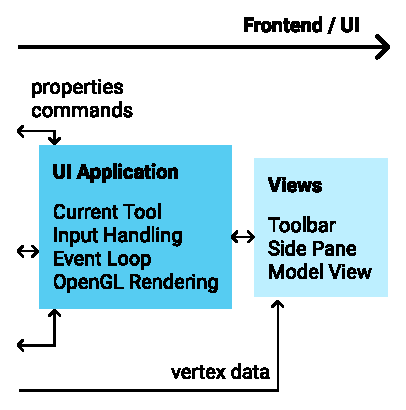
\includegraphics[scale=0.9]{images/architecture_ui.eps}}
	\caption{An overview of the Pepr3D UI architecture, based on Figure~\ref{fig:architecture}.}
	\label{fig:architecture_ui}
\end{figure}
\vspace{-1.5em}
\section{Introduction}

We did not want to reinvent the wheel, so we investigated how other developers recommend to implement user interfaces.
In our case, we have \emph{3D rendering}, i.e., displaying the 3D model, and \emph{UI widgets}, i.e., the windows, buttons, check boxes, text labels, etc.
Here we describe what we found important to understand.

\subsection{Existing patterns}

Let us have a look at existing generic UI architectural patterns.
A detailed overview of them was written for example by Derek Greer\footnote{https://lostechies.com/derekgreer/2007/08/25/interactive-application-architecture/}.
The most common pattern is called Model-View-Controller (MVC), where \emph{model} is a state, \emph{views} visualize the state, and \emph{controllers} react to user input to manipulate the model.
The MVC pattern got so famous that there are a lot of alternatives nowadays based on the similar principles, like Model-View-Viewmodel (MVVM), Model-View-Presenter (MVP), or Presentation-Abstraction-Control (PAC).

But we can go even further: Johannes Norneby mentions\footnote{http://www.johno.se/book/immvc.html} a common paradigm of UI, which he objects is \emph{not valid}: \emph{``The user interface and / or visualization of any program is inherently stateful.''}
He objects that this is a broken paradigm and devotes his book into explaining the so called \emph{immediate user interface}, which instead provides a \emph{stateless} alternative to rendering UI.
% Nowadays, there exist various libraries and frameworks based on this idea, the most well known probably being ImGUI\footnote{https://github.com/ocornut/imgui} supported by large companies such as Blizzard Entertainment.

The main difference between \emph{immediate} and \emph{retained} modes is that in the latter, the visualization library \emph{retains} internally a complete model (state) of objects to be rendered, while the former is procedural and redrawn every frame.\footnote{http://msdn.microsoft.com/en-us/library/windows/desktop/ff684178(v=vs.85).aspx}
The major benefit of a stateless immediate UI is the ability to maintain and reuse it much easier.
Norneby suggests that every \emph{view} should be as \emph{pure} as possible, meaning that in languages like C++, all views should in fact be \emph{free functions}.

\subsection{Immediate vs. retained}

Even when one sticks to MVC principles, there does not seem to be a consensus for which applications one should prefer the \emph{retained} mode over \emph{immediate} and vice versa.
At its core, MVC principles can be used in both of them.
Norneby goes as far as saying that MVC \emph{and} immediate UI are two implicitly connected concepts.
Arguments were made\footnote{https://gamedev.stackexchange.com/questions/24103/immediate-gui-yae-or-nay} for both approaches without a clear winner.

The main downside of retained UI is the necessity to maintain a UI state.
This often leads to complex libraries that are difficult to learn to work with and introduces out-of-sync bugs that are hard to fix.
This is why video game and interactive applications developers (including Blizzard Entertainment) support immediate UI, because it \emph{interlocks} the application data and the current state of the UI, meaning the state and UI never get ouf of sync.
The libraries are also usually very simple to use.

The main downside of immediate UI is a poor separation of logic and presentation and the necessity to rerender the UI more often.
What developers at uiink\footnote{https://uiink.com/articles/data-driven-immediate-mode-ui/} suggest is to just use the best of the both worlds.
And it is not different from what Norneby actually proposed in his never-finished book.
We should only use immediate UI in the actual \emph{views}, which are just free functions procedurally explaining how the UI should be rendered each frame.
The rest of the application should know nothing about immediate UI.
In theory, we should be able to swap immediate UI and retained UI, or use both of them together without the need to touch the rest of the application.

\subsection{Real-time rendering}

In Pepr3D, a regular user interface with a few buttons and texts is not enough.
We primarily need real-time 3D rendering and manipulation of the 3D model that the user is editing.
Hence the whole user interface needs to take this into account and should be primarily based on real-time rendering.

As already mentioned, real-time applications such as video games favor immediate UI.
They need to rerender the whole screen all the time anyway.
For Pepr3D, it is perfectly possible to make immediate UI a part of the renderer.

\subsection{Presentation separated from logic}

Nowadays, a lot of UI is being developed for web applications.
We can investigate the most used frameworks and libraries for single-page applications\footnote{React: https://reactjs.org/, Angular: https://angular.io/, Vue.js: https://vuejs.org/}: React by Facebook, Angular by Google, or Vue.js.

We observed that these tend to follow the principle that a \emph{view should be just a thin front-facing layer only responsible for displaying data}.
Calculations and data manipulation should be done in other parts of the application.

It is not a surprise that even Qt\footnote{https://www.qt.io/}, a widely used C++ UI framework, encourages people to eliminate data consistency problems by using separate \emph{views}.\footnote{http://doc.qt.io/qt-5/modelview.html}
Even though there are so many different UI libraries and frameworks, they all seem to share the same common principles about the separation of presentation.

\subsection{Internationalization and accessibility}

There are many other observations one can make when studying existing applications that heavily rely on user interface.
A lot of energy has been invested into creating standards and guidelines for them.
It is not in the scope of this work to list all details about building good user interfaces, but we should still mention at least two more concepts: internationalization and accessibility.

Typically, when applications are used by users from different countries, the UI needs to support \emph{internationalization} (abbreviated as \emph{i18n})\footnote{https://blog.mozilla.org/l10n/2011/12/14/i18n-vs-l10n-whats-the-diff/}, i.e., different languages, number formats, time formats, etc.

Applications should also be \emph{accessible} (accessibility, abbr. \emph{a11y}), meaning they should support keyboard navigation for people who cannot use mouse, screen readers for people who are blind, high contrast themes for people with worse eyesight or color blind users, etc.
Especially in the ``web world'', there exist important accessibility guidelines called WCAG.\footnote{https://www.w3.org/WAI/standards-guidelines/wcag/}

\section{Our requirements}\label{sec:uireqs}

Based on the observations made in the previous section, on the expected usage of our application, and on general advice gathered from Vojtěch Bubník from Prusa Research s.r.o., we decided on the following set of requirements for the user interface of Pepr3D.

The user interface of Pepr3D and the library we are going to use for it should:
%
\begin{enumerate}
\setlength\itemsep{0em}
\item separate presentation from application logic, i.e., in theory, we should be able to easily replace the UI with another one, should it be necessary,
\item support real-time 3D rendering of the 3D model, provide an easy-to-use abstraction, e.g., for rendering 3D primitives, using custom shaders with uniforms, uploading textures to the GPU, keeping constant framerate, etc.,
\item look visually good and allow us to unify the design of the 3D rendering part and the rest (toolbar, controls, etc.), e.g., by supporting custom themes,
\item be cross-platform at least on desktop (Windows, Mac, Linux), ideally on tablets as well (Android, iOS), i.e., the ``cross-platformity'' of Pepr3D should not be limited by the UI library,
\item support keyboard navigation, e.g., tabbing to buttons and input elements, using keyboard to enter values,
\item support high DPI, e.g., Apple Retina displays, Microsoft Windows scaling,
\item support asynchronous events, e.g., long calculations on background should not affect the UI thread,
\item support internationalization including plurals, time formats, UTF-8, and
\item the license of such library should be as least restrictive as possible, e.g., allowing commercial usage and redistribution, should the development of Pepr3D continue after this initial school project is finished.
\end{enumerate}

\section{Choosing a 3D rendering library}

There are many cross-platform C++ libraries for 3D rendering and for creating user interfaces.
Picking the right ones for Pepr3D is not an easy task.
Fortunately, as we built a list of requirements in the previous section, we can easily disregard the libraries that do not conform to our requirements.
Let us now describe how we chose a library for the 3D rendering part of Pepr3D.

\medskip

In order to support multiple platforms and even older computers, we decided to use OpenGL rendering API instead of Microsoft DirectX or alternatives like Vulkan.
We cannot use OpenGL on its own as we need a library to handle cross-platform windows, contexts, keyboard and mouse inputs, etc., so it is necessary to find a library that can help us with that.

There are many libraries like SDL, GLFW, Cinder, Ogre3D, or bgfx,\footnote{https://www.libsdl.org/, https://www.glfw.org/, https://libcinder.org/, https://www.ogre3d.org/, https://github.com/bkaradzic/bgfx} and some UI libraries like Qt can also help with that.
Some of these libraries depend on others from the list, for example bgfx uses SDL for windows and input handling, and Cinder uses native code for Windows and OS X but GLFW on Linux.

We had previous knowledge of Cinder and bgfx.
The other libraries we examined did not seem to provide any advantages over these two, either because they were already included in the two, or because they were too heavy.

We found that Cinder conforms to our requirements better than bgfx:
Cinder has built-in high DPI support, font rendering, event loop for asynchronous events, a big set of tutorials and examples, and much more.
We have decided to choose \textbf{Cinder} as the library for real-time 3D rendering.

\section{Choosing a UI widgets library}

Now that we know what library to use for 3D rendering, we need to choose a way to display \emph{widgets} such as toolbars, buttons, check boxes, or text labels.
Again, there are famous cross-platform libraries that already exist for these purposes, so it would not make much sense to make our custom solution.

\subsection{Why not wxWidgets nor GTK$+$}

We should definitely mention retained UI libraries wxWidgets and GTK+.\footnote{https://www.wxwidgets.org/, https://www.gtk.org/}
They are both cross-platform and used by famous software like GIMP or Audacity.
Unfortunately, we found major flaws with both of them.

Regarding wxWidgets, we did not really like its default appearance.
It uses native controls where possible making theming very limited and also undocumented.
Hence, we would not be able to easily unify the design of the 3D view and the rest of the application.
Also, only desktop is supported.

Regarding GTK+, they do support theming up to some degree, they also added OpenGL rendering widgets a few years ago.
Making Cinder and GTK+ work together would probably cost us some effort as we did not find any already working solution.
The problem with GTK+ is that a lot of developers who actually use it are not satisfied and warn others about using it.\footnote{https://davmac.wordpress.com/2016/07/05/why-do-we-keep-building-rotten-foundations/}$^{,}$\footnote{https://fosspost.org/opinions/are-gtk-developers-destroying-linux-desktop-with-their-plans}$^{,}$\footnote{https://www.reddit.com/r/linuxmasterrace/comments/7xkcwo/}

They say that GTK+ documentation is very bad and that different versions of GTK+ break existing applications, extensions, and themes, because the API and ABI is changing rapidly providing no guarantees.
It did not seem that using GTK+ for Pepr3D would be a good long-term idea should anyone continue with its development in the future.

\subsection{Qt}

We have already mentioned Qt on previous pages of this specification.
It is a rather large actively-developed library providing a lot of features including their own internationalization solutions and so on.
Qt conforms to all our requirements stated in the previous section.
There are two major drawbacks with Qt: its controversial licenses\footnote{https://www1.qt.io/licensing-comparison/} and its huge size.

The licensing is controversial because either one can pay for the commercial license, or one can use the LGPLV3 one, but it requires dynamic linking, providing users the ability to relink the application, and also the necessity to deliver complete Qt source codes to users including all changes made if any.
The huge size is also an issue, because using only the basics of Qt (widgets, GUI, and core) is already around 17 megabytes in libraries, which together with Cinder would lead to a very large size of the final Pepr3D application.
It is also uncertain whether it would be a good idea to use Cinder together with Qt, so we would possibly need to rely on a different library.

\subsection{UI libraries for OpenGL}

There are also libraries that do not use native controls at all, but rather generate draw instructions and lists that can be used by renderers like OpenGL directly.
The libraries itself do not handle window creation, native calls to operating systems, etc.
Users of such a library need to bind the input handling and draw commands of these libraries to their own OpenGL/DirectX/other renderer.
In our case, we would need to connect the library to Cinder, which handles windows, inputs, and rendering itself.

There are many such libraries, e.g., Dear ImGui, Nuklear, NanoGUI, and FlatUI.\footnote{https://github.com/ocornut/imgui, https://github.com/vurtun/nuklear, https://github.com/wjakob/nanogui, https://github.com/google/flatui}
While some of them like NanoGUI and FlatUI seem to be rather small, without that many users, and not under active development, Nuklear and Dear ImGui are still under active development and maintenance.

Nuklear is an ANSI C header-only library with a C API and C naming conventions.
We did not manage to find existing Cinder--Nuklear bindings that we would be able to use, so we would need to develop them ourselves.
For this reason, we did not continue investigating Nuklear, because we found an alternative.

Dear ImGui (or just ImGui) is a modern bloat-free C++11 library that we already mentioned in the previous sections.
It is backed by large companies like Blizzard Entertainment or NADEO.
Its community is very active providing different bindings for different renderers and libraries including Cinder.
It is easily themable and we have created a prototype with completely custom controls.

\subsection{Final decisions}

For our final decisions, we have selected two libraries: \textbf{Qt} and \textbf{ImGui}.
When looking at our requirements from Section~\ref{sec:uireqs} (numbering refers to Section~\ref{sec:uireqs}):
%
\begin{enumerate}
\setlength\itemsep{0em}
\item separation can easily be achieved in both using Views and Models,
\item OpenGL rendering is implicit in ImGui, there is a widget in Qt,
\item theming in Qt: QSS stylesheets, in ImGui: styles and custom drawing,
\item both are cross-platform even on mobile devices,
\item both support keyboard navigation, ImGui since version 1.60,
\item high DPI possible in Qt, for ImGui we can use Cinder high DPI support,
\item Qt has its own thread pool, signals, and promises, for ImGui we can use C++11 and Cinder/ASIO event loop using dispatchAsync,
\item Qt has its own i18n support, for ImGui we can use PO files and gettext\footnote{Free i18n system commonly used on Linux, see https://www.gnu.org/software/gettext/} together with a translation editor, e.g., open-source PoEdit\footnote{https://poedit.net/},
\item Qt is unfortunately commercial or LGPLV3 (see above), ImGui has much less restrictive MIT License.
\end{enumerate}

As we can see, there is no clear winner: both libraries have positive and negative attributes.
In fact, Qt and ImGui are very different.
Qt is a large retained UI library and ImGui is a small bloat-free immediate UI library.

Using Qt together with Cinder is rather questionable as they both overlap in certain areas like window management and event handling.
Whereas ImGui needs a renderer and a window handler anyway, so using it with Cinder seems to be a good idea.
ImGui is much closer related to the actual OpenGL rendering and offers us quite a bit more flexibility.
It also has a very simple source code that one can read in an evening, meaning we can actually learn a lot about how such a library is made.

We think that Qt would probably be an unecessary huge piece of middleware that we would have to learn just for the sake of this project.
We have decided to use \textbf{ImGui} for the Pepr3D user interface.

\section{Final proposal}

In Section~\ref{sec:wireframe} and in Figure~\ref{fig:wireframe}, we have already proposed a wireframe of Pepr3D and explained why we find it reasonable and easy to use.
In this chapter, we explained our requirements and investigated existing patterns for actually implementing the UI.
Let us now propose how we can use these together.

\subsection{Overview}

We propose to divide the Pepr3D UI into the following main parts that correspond to the wireframe in Figure~\ref{fig:wireframe} and to Figure~\ref{fig:uioverview}:
%
\begin{itemize}
\setlength\itemsep{0em}
\item a \textbf{toolbar} with toggleable buttons representing tools, undo/redo, etc., implemented as an ImGui widget rendered with Cinder,
\item a \textbf{side pane} with buttons, checkboxes, sliders, etc., representing configuration of the currently selected tool, also implemented as an ImGui widget rendered with Cinder,
\item and a \textbf{model view} with the 3D model which the user can rotate, zoom, paint on it, etc., implemented in OpenGL using Cinder.
\end{itemize}

Even though the toolbar and side pane are to be implemented in ImGui, they will in fact be rendered using Cinder and OpenGL as well.
The whole window is managed by Cinder and has a single large OpenGL drawing context.

\begin{figure}[h]
	\centering
	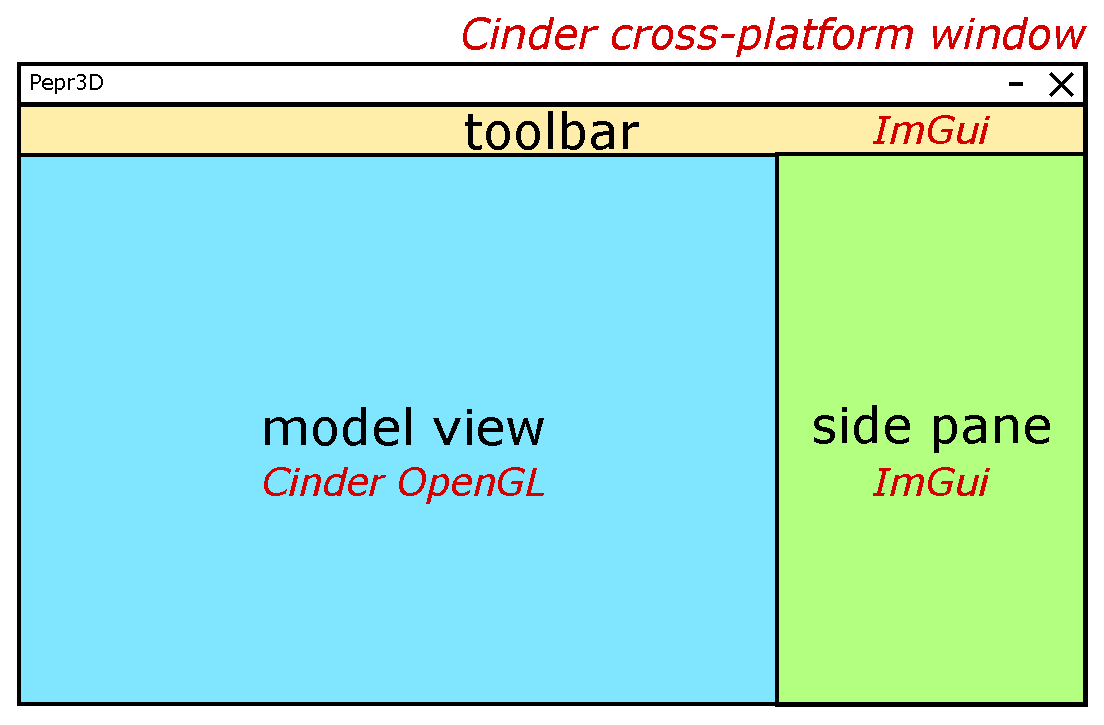
\includegraphics[scale=0.65]{images/uioverview.eps}
	\caption{An overview of the Pepr3D UI.}
	\label{fig:uioverview}
\end{figure}

\vspace{-1em}
\subsection{Stateless views / widgets}

Inspired by the immediate UI advice, we propose to use \emph{stateless views} that will be responsible for drawing the UI.
We can implement these views as C++ free functions without encapsulating them in any classes.
This is a common pattern in C++, e.g., in the standard library, because unlike in languages like Java and C\#, functions in C++ do not need to be enclosed in classes.

Having stateless views means that we do not have to program any explicit synchronization between the UI and the backend.
Whenever we rerender the UI, it will be rendered with the newest data.
We should try to avoid retained state in the UI as much as possible, but it might be necessary in specific situations, e.g., for scrollbar positions or complex calculations that we do not want to do each frame.
The ImGui library provides ways for retaining states.
Where necessary, we can also use regular C++ classes and their instances.

There is also a huge ImGui community at GitHub, where we can find both simple and complex widgets available from other users of the library.
We should aim at making our UI composed of reusable ImGui widgets.

\subsection{Internationalization and accessibility}

It should be possible to change a language of the application.
For this purpose, we propose to use PO files that are used by a lot of Linux distributions and applications including PHP.
Loading the PO files can be handled by lightweight libraries that already exist and are suitable for our project, at a first glance sporit-po\footnote{https://github.com/cbeck88/spirit-po} looks perfect for our purposes.
The files themselves can be generated from source codes and translated using for example the already mentioned PoEdit.

The UI should provide basic keyboard navigation including hotkeys (shortcuts).
It is especially important that the currently selected tool can be changed by pressing a single key on a keyboard.
We also considered adding a radial menu to a specific mouse button (e.g., middle button click), but it is not a top priority.
The default theme of Pepr3D should provide sufficient contrast and it should be easy to see which tool is selected and what options are enabled.


% Describe unit testing, CircleCI on GitHub and manual testing of each tool
\chapter{Testing}

In this chapter we describe our testing pipeline. We have several ways how to test if the program behaves correctly. Namely:

\begin{itemize}
\item \textbf{Unit tests} -- the basic testing of several components of Pepr3D. The unit tests are small use-cases crafted to test each functionality of the object individually. The tests are great for catching quick and stateless errors but do not provide any information about more complex operations.

\item \textbf{Manual tests} -- because of the simplicity of unit tests, we have several written manual tests for each tool in Pepr3D. These are executed manually by the person doing the predefined operations, and checking the result against the expected result.

\item \textbf{Continuous integration} -- our Git repository is equipped with Continuous Integration software. This ensures that every pull request and merge is compilable, which ensures every commit in the \textit{master} branch is compilable and runs the unit tests automatically. The merge will not be executed if either of these conditions fail.
\end{itemize}

In the following sections, we explain these types of tests in detail, as well as provide the descriptions of the manual tests.

\section{Unit tests}

Unit testing is probably the most common way to automatically test software. As such, we will not explain in detail the benefits of this procedure. We use Google Test library \footnote{https://github.com/google/googletest} as it is one of the best C++ testing frameworks we have found. Several of our team members also already had experience with Google Test.

For better navigation in the code base, we decided to follow the common naming convention: for class \texttt{CommandManager}, we have \texttt{CommandManager.h} and \texttt{CommandManager.cpp} as the implementation files. Now to test this class, we add \texttt{CommandManager.test.cpp} file and program all \texttt{CommandManager} into this file. This makes searching for tests very easy.

\subsection{Library test}

The test \texttt{libraries.test.cpp} is a special case among our unit tests. As the name suggests, this test checks whether our 3rd party libraries are setup correctly. This test should always succeed if it is compiled. If it does not get compiled or linked, the libraries were set up incorrectly.

\subsection{Class tests}

All of the other tests are the "standard" type of tests -- testing the public methods of the class. We will not describe each of the tests individually, since each test has a documentation comment inside describing what the test does, as well as a fitting name. 

The general structure of the unit tests is cumulative -- this means that if the first test fails, there is a high chance all of the the following tests will fail too. The advantage of this approach is clear once you imagine a different sorting of the tests. If the first test was a complicated behaviour of the class, the test will fail not only if the behaviour is incorrect, but also if the initialization of the class is wrong. This is bad, because the programmer fixing the test will not immediately know which part of the class is incorrect.

\section{Manual tests}

In this section we describe the reasoning behind manual testing. We also list all of the manual tests the team has accumulated during the development.

\section{Continuous integration}

Continuous integration is a software engineering term used to describe the work flow of a team based project, which is based on merging the work of many individuals into a main stream often \footnote{https://en.wikipedia.org/wiki/Continuous\_integration}. In particular, \textit{Circle CI} is a free service which can be integrated into GitHub's interface, which allows the users of the repository to perform all kinds of checks and tests before the code is merged into a branch (most commonly the \textit{master branch}.

We performed three checks before allowing the merge into a different branch, namely:

\begin{itemize}
\item \textbf{clang-format check} -- by running clang-format on the whole codebase and comparing it to the one before the run, the software determined if all of the code is properly aligned and follows our coding standards. This benefits us in two ways. Firstly, we minimize the number of git conflicts, because the code is properly formatted. Secondly, this makes the code uniform and such it removes any personal preference in coding styles. The second property is important because it makes reading the code much more programmer friendly -- once formatted, you cannot distinguish between your and the others' code, which makes reading it much easier, as you are not bothered by different standards of formatting.

\item \textbf{ability to compile} -- code that does not compile is very dangerous in a repository, especially in the \textit{master} branch. If we need to step back in the \textit{master} branch history to trace the origins of a bug, we want to be building the program and testing it for the bug to find the commit that introduced the bug. If we run into code that does not compile, this methodology is much harder to execute. Our check was performed on a Linux machine, so it had another positive outcome for the team. The team developed on MSVC as our main target was the Windows OS. However, g++ has different and sometime better checking for errors than MSVC, which allowed us to catch some mistakes during compile time on Linux, which we did not see on MSVC.

\item \textbf{unit testing} -- the last check the code needed to pass was the unit tests, which we already discussed. This point is rather simple, if the tests fail, the added code would break Pepr3D, and as such should not be committed.

\end{itemize}

We used Circle CI \footnote{https://circleci.com/} and integrated the service into GitHub.

% Describe how to build Pepr3D from scratch
\chapter{Building the project}
\label{ch:build}

In this chapter, we explain how Pepr3D can be built from the source codes.
We assume some knowledge of build systems, compilers, and operating systems as this is a guide for developers.

\section{Building on Windows}

We explain how the 64-bit Pepr3D can be built on Windows 8 and 10, which are the officially supported platforms.

\subsection{Repository}

First of all, the official Pepr3D git repository has to be cloned.
This requires git to be installed on the machine and then cloning the repository using the following command in the Windows command line:

\begin{lstlisting}[
    basicstyle=\scriptsize\ttfamily,language=command.com
]
git clone --recurse-submodules -j8 https://github.com/tomasiser/pepr3d.git
\end{lstlisting}

If you have already accidentally cloned without submodules, run this command from the root directory of this repo:

\begin{lstlisting}[
    language=command.com
]
git submodule update --init --recursive
\end{lstlisting}

\subsection{Dependencies}

The following dependencies have to be downloaded and/or installed on the machine according to these steps:

\begin{enumerate}
\item Download and install the latest \textbf{CMake} from https://cmake.org/.
\item Download and install either \textbf{Visual Studio 2017} (Community version is enough) or alternatively only \textbf{Build Tools for Visual Studio 2017}. Both can be found at https://visualstudio.microsoft.com/downloads/.
\item Download and install \textbf{CGAL} from https://www.cgal.org/download/windows.html. Make sure \texttt{CGAL\_DIR} environment variable is set to the installed CGAL path, which is done by default when using the official installer.
\item Download and install \textbf{Boost} from https://www.boost.org/. You can either build Boost yourself or download pre-built binaries for the 14.1 toolset. Make sure to point \texttt{BOOST\_ROOT} environment variable to the installed Boost path.
\item We use our own built version of \textbf{Assimp} from the latest \texttt{master} branch. Either build Assimp yourself from https://github.com/assimp/assimp, or download and unzip our prebuilt version\footnote{https://github.com/tomasiser/pepr3d/releases/download/v1.0/Assimp\_for\_Pepr3D.zip}. Our version is built with two \texttt{.dll}, one for Debug and one for Release. Do not mix them up! Make sure to point \texttt{ASSIMP\_ROOT} environment variable to the Assimp directory.
\item Download \textbf{Freetype} from https://github.com/ubawurinna/freetype-windows-binaries, preferably version 2.9.1. After downloading, it is \emph{necessary} to rename the \texttt{win64} subdirectory to \texttt{lib}. Make sure to point \texttt{FREETYPE\_DIR} to the Freetype directory.
\end{enumerate}

All other libraries are part of the Pepr3D repository and will be built automatically by our build system.

\subsection{Building}

From the root directory of the cloned repository, run the following from the command line, which creates a new \texttt{build} directory and runs CMake inside:

\begin{lstlisting}[
    language=command.com
]
mkdir build
cd build
cmake -G"Visual Studio 15 2017 Win64" ..
\end{lstlisting}

Now the build project is prepared inside the \texttt{build} subdirectory and we can now open \texttt{build/pepr3d.sln} in the Visual Studio 2017 application and compile Pepr3D from there.

\paragraph{Building from command line}
Alternatively, we can build Pepr3D from the command line using the build tools. We have to start \textbf{MSBuild Command Prompt for VS2017} or \textbf{Developer Command Prompt for VS 2017} from Start Menu, or we can also start the command prompt from a standard command line using:

\begin{lstlisting}[
    language=command.com
]
%comspec% /k "C:\Program Files (x86)\Microsoft Visual Studio\2017\Community\Common7\Tools\VsDevCmd.bat"
\end{lstlisting}

In the Visual Studio command prompt, we can build Pepr3D using:

\begin{lstlisting}[
    language=command.com
]
msbuild pepr3d.sln /m
\end{lstlisting}

\subsection{Running}

The executable of Pepr3D should be located in \texttt{build/pepr3d/Debug/pepr3d.exe} (or \texttt{Release} instead of \texttt{Debug}).

After building in Visual Studio, we have to make sure the appropriate \texttt{.dll} files are copied next to the executables.
If you used Visual Studio 2017 application to build it, some of the \texttt{.dll} files should be automatically copied to the executable directory.
If you used command line to build, you need to copy \texttt{libgmp-10.dll}, \texttt{libmpfr-4.dll}, and \texttt{assimp-vc140-mt.dll} manually from the \texttt{build/} directory to the same directory as \texttt{pepr3d.exe}.

\paragraph{Copying correct Assimp \texttt{.dll}}
Note that by default, the Release version of Assimp \texttt{.dll} is copied.
If you built a Debug version of Pepr3D, you need to replace \texttt{assimp-vc140-mt.dll} by the file located in the directory where you unziped our Assimp library.
The Debug library is in the \texttt{bin/x64-Debug} subdirectory of Assimp instead of in \texttt{bin/x64}.
If you built Assimp on your own, you need to compile it in the same Debug or Release as Pepr3D.

\paragraph{Copying Freetype \texttt{.dll}}
If you do not have \texttt{freetype.dll} as a part of your operating system already, you also need to copy this file next to the executable from the \texttt{lib} subdirectory of the Freetype you downloaded as described in the Dependencies subsection.

\paragraph{Running unit tests}
By default, the Debug executable of all Pepr3D unit tests is build into \texttt{build/Debug/pepr3dtests.exe}.
It is necessary to also copy the \texttt{.dll} files there.

\section{Building on Linux / Docker container}

There is a possibility to build Pepr3D on Linux systems, but please note that is in only supported for verifying that the source codes do compile as necessary for continuous integration (Section~\ref{sec:ci}).
It is not indended for running and using Pepr3D in release.

We have a Linux Docker container\footnote{https://www.docker.com/resources/what-container} in our special repository at GitHub: https://github.com/tomasiser/docker-cinder.
The \texttt{latest} image setups a Debian environment to build Cinder applications.
The \texttt{prebuilt} image actually builds Cinder on top of the \texttt{latest} image.
Pepr3D can be built in the \texttt{prebuilt} container by running \texttt{cmake} and \texttt{make} commands from the Pepr3D repository.

Note that in order to compile Pepr3D using the container, one needs to have at least a minimal experience with Docker.
We advise to follow the tutorials on the official Docker website\footnote{https://docs.docker.com/get-started/}.

% III. PROGRESS OF IMPLEMENTATION
\part{Progress and results}

% chronologický popis průběhu prací na projektu
\chapter{Progress of implementation}

In this chapter we first cover the tasks and responsibilities of each of the team members. Then we outline the progress of the implementation of this project.

\section{Responsibilities}
\label{sec:responsibilities}

Here we list the members of the team alphabetically and summarize all the work each of them has done over the course of the project.

\subsection{Bc. Štěpán Hojdar}
\begin{itemize}
\item Implementation of the Geometry class as a data structure, which entails both computational geometry (colouring the triangles, etc.) and rendering capabilities (creating buffers for OpenGL). Testing and integrating the CGAL library into the project and using this library to perform the computational geometry.
\item Implementing the following tools both on the backend and the frontend: bucket painter, manual segmentation and automatic segmentation.
\item Researching a way to convert a font file (.ttf) into a 2D triangle mesh, implementing the FontRasterizer class and implementing the basics of the text tool, using this knowledge.
\item Serializing and deserializing our data using the Cinder library, which allows us to save work in progress as a .p3d file.
\item Writing a major part of both the specification and the documentation.
\end{itemize}

\subsection{Bc. Tomáš Iser}
\begin{itemize}
\item The majority of the user interface of the application, including the design of the GUI, the architectural design of the backend of the UI.
\item Small widgets -- wrappers around Dear ImGui calls to make it easier to use for the rest of the team while developing the UI.
\item The color palette editor, shortcuts, correctly scaling and rotating the model, all of the display options (wireframe, two zoom options), tooltips, dialogs, error handling and logging and application settings.
\item Prototyping, testing and integrating the Cinder and Dear ImGui libraries which we based the project on.
\item The Export Assistant (the visualization part) and Triangle Painter tools.
\item Writing a part of both the specification and the documentation (UI, build).
\item Connecting our GitHub repository to Circle CI, which is a continuous integration service based on linux. We used the CI throughout the whole process, which made sure every single merge into the master branch was buildable and passed all unit tests.
\end{itemize}

\subsection{Bc. Jindřich Pikora}
\begin{itemize}
\item Communication with Prusa Research s.r.o., including several meetings with our contact in Prusa Research.
\item Testing and familiarizing himself with the FDM printing in practice, printing a lot of test subjects to measure the printer's capabilities and downsides, to note during our export development.
\item Testing and integrating the Assimp library into the project.
\item Implementing the whole import process, with mesh pre-processing, simplification and repairs provided by the Assimp library.
\item Implementing the whole export process, researching and developing a usable heuristic to make the process smoother and less error prone. Testing the export by physically printing the results on our printer.
\end{itemize}

\subsection{Bc. Luis Sanchez}
\begin{itemize}
\item Setting up the project environment using CMake, making sure all our libraries compile and link correctly.
\item Designing and implementing the whole command architecture, with functioning undo and redo operations on the geometry data.
\item Implementing the Brush and Text tool backend and frontend, requiring long and extensive research and developing a brand new way to solve this problem, which we did not find in any available literature or research papers.
\item Modifying and extending the Geometry data structure to allow for custom triangle subdivisions.
\item Performing complex operations using the CGAL library on the modified Geometry in order to make the brush work correctly.
\item Modifying the rest of the tools to be able to work on the new custom modified geometry, as well as to allow it to correctly export and serialize as a .p3d project.
\end{itemize}

\section{Timeline of the implementation}

In this section, we describe the process of implementing this project from start to finish. We start by explaining the project setup, rules and other measures we employed to get more productive, then we describe the process itself.

\subsection{Rules and project setup}

\subsubsection{Team management}
To manage the work in the team, we set several goals. We met regularly each week with our supervisor, and had a structured meeting. The first part of the meeting had each of us tell the rest of the team what we worked on the last week, describe what went well and if/where we got stuck. This had two effects -- firstly, it allowed us to help the stuck member and not waste too much time, and secondly, this made sure that all the team members are up to date with the progress of the whole project, which motivated further progress. The second part of the meeting had us setting goals for the next week, assigning clear and doable tasks to each team member, which would get reviewed on the next meeting. Each meeting took around an hour, including a general discussion after these two structured points.

\subsubsection{Git repository}
The second major part of the teamwork was our git repository, which we setup on GitHub \footnote{https://github.com}. We employed several measures to ensure the quality of the code and to avoid issues like a master branch that cannot be compiled.

Firstly, we disabled any way to push directly into the master branch. This had the effect that every contribution has to go through GitHub's \textbf{pull request} mechanism. We also set the pull request merge to require one approving review. This means that for each merge (and therefore commit), two people were required to read the code - the one who wrote and tested it, and the reviewer, whose only job was to go over it, try to compile it and point out any weak programming in the code.

Secondly, as we already mentioned in the previous section, one of our team member set up a continuous integration service, called Circle CI \footnote{https://circleci.com/}. We required the CI to be run on every pull request that was sent towards the master branch. The CI would notify us if the pull request either did not compile, or did not pass all of the unit tests. Because Circle CI utilizes a linux server to build the program, it also meant that we would be sure it compiles on both Windows and Linux all the time.

Last but not least, we also made sure to set the CI to check the code formatting. We have discussed and configured the clang-format tool \footnote{https://clang.llvm.org/docs/ClangFormat.html} to format our code in the same way, to avoid mixed coding standards. If the code was not formatted correctly, the pull request wouldn't go through.

These two measures helped us immensely and made the code more reliable in the long run.

\subsection{The process of the implementation}

Here, we will go over the process of the implementation, week by week, as can be seen in the git log, starting on 01.10.2018, when we sent the specification to the committee.

\subsubsection{01.10. - 08.10.}

By now, we have had a functioning repository, since we used it to create the specification as well. We also had the continuous integration working. This week we started to implement the basic functionality, so far in separate projects, because the CMake of the whole project was not finished yet, so the project didn't include all the necessary libraries (e.g. CGAL or Assimp). The application was running, but there were no responses to the buttons and nothing to render. The basics of the command manager also got implemented, even though they would wait for another month before being applied to the Geometry class.

\subsubsection{09.10. - 16.10.}

This week we added the basic Geometry class and ray-shooting capabilities using CGAL, because the CMake finally accepted the CGAL library. We started rendering the geometry in the ModelView (for now a triangle) and could shoot rays.

\subsubsection{17.10. - 24.10.}

This week the Assimp library got added into CMake, and the ModelImporter was merged, which meant we could import models into the geometry, and render them in the ModelView window. We had begun to try to debug normals of the mesh Assimp gave us, which will take a bit more time, since the library is not clear on what it does in the documentation.

\subsubsection{25.10. - 1.11.}

We added ray-casting from the model view, which happens on a mouse click, which allowed us to finally get the Triangle Painter functionality to be complete -- we could click on a triangle and change its color. We also started adding unit testing, for now only for the Geometry class. Drag and drop was now also a supported way to load a model. We redid the color palette as a integer based data structure, instead of RGB color notation.

\subsubsection{2.11. - 9.11.}

This week we struggled with the CGAL library and managed to get the bucket painter to do a breath-first-search over the model. We also modified the shader to accept the the colors as integers and then a color palette array, which allows for real-time color swapping done in the color palette.

\subsubsection{10.11. - 16.11.}

Assimp finally stopped loading degenerate triangles, which was due to the wrong setup and what we believe is a bug in the library, which we solved by double checking the output. We also extended the bucket painter tool to allow for stopping on different criteria (like edge sharpness or color), and modified the Command Manager to be more memory friendly and customizable. The UI received a highlight for the hovered triangle, and an editable color palette. We also added some basic error handling, bucket painter UI, and made the Undo and Redo work on bucket painter.

\subsubsection{17.11. - 23.11.}

Geometry got a big refactoring, which removed a lot of lower quality code that got detected in a code review and fixed a few warnings that were showing up on g++ and not on MSVC. The camera handling got improved and now always fit the model, instead of always pointing in the same direction. Bucket painter got a prettier UI and better stopping criteria. A working export is finished, and the team notices a few cases, which break the export. Research and testing will continue in the following weeks to try to find a way to make the export more robust.

\subsubsection{24.11. - 1.12.}

Loading a new geometry is now done in parallel, using a threadpool. Brush development is starting and the backend for automatic segmentation is done. The frontend for automatic segmentation is developed, and a new way of rendering custom colors is added. Work also starts on implementing the manual segmentation. Tools that are disabled (because the user loaded a non-valid model) are now greyed out and cannot be selected. Dialogs get implemented to show the user progress while loading a new model.

\subsubsection{2.12. - 9.12.}

Manual segmentation is done, but the team is not happy with the handling. We discuss the behaviour during a meeting and the behaviour is changed to a different one, which we are happy with. UI Tooltips get implemented, both for Tools and for the tool configuration. Work is also starting on serializing and deserializing the geometry. The brush starts to work, but is really slow and needs optimization.

\subsubsection{10.12. - 17.12.}

Brush is still getting improved, now is able to undo and redo the operations. Serializing and deserializing is done, the unsaved asterisk mark gets added, as well as \textit{Save} and \textit{Save as} options. The OpenGL buffers get redone, so they do not recalculate every frame. A few crashes are fixed and a lot of refactoring is done on the existing code.

\subsubsection{18.12. - 01.01.2019}

Hotkeys are updated, more tooltips get added. The brush is getting UI settings (like size of the brush) and gets a highlight around the cursor. It's Christmas, so work gets slowed down. Work on export is done, using the CGAL library to determine the thickness is accepted by the team as a viable way to prevent the majority of bugs.

\subsubsection{01.01. - 08.01.}

Font conversion from a .ttf into triangle meshes gets researched and added. The UI is getting final polishing, spell-checking and gets a scrollbar. The new geometry from Brush is getting fixed in other already existing Tools, and a lot of error dialogs and crash prevention is done. Logging is improved and exception handling for multi-threaded load and import is fixed.

\subsubsection{09.01. - 16.01.}

Export is getting reviewed, brush is getting reviewed and bug fixed. The functions that convert the Brush tool into the Text tool get added. The team decides to start writing this document, since the program is almost feature complete.

\subsubsection{17.01. - 24.01.}

This document gets started. The brush is still getting polished and the export is getting merged into master. The attention of half of the team is shifted towards this document, while the remaining two members finish the few remaining features of the program.

\subsubsection{25.01. - 01.02.}

Documentation is being written, mostly by Štěpán as other team members need to focus on fixing the remaining bugs. After meeting with Oskar, we decide to implement the Export Assistant tool to improve the export process significantly.

\subsubsection{02.02. - 09.02.}

The Export Assistant tool is finished, exporting is being verified. The remaining bug in the Brush tool is being debugged and fixed. The documentation is being finished. We focus on the user documentation and finding a good model to showcase the results of our work.

% Compare our result with the minimal implementation we specified. And with the advanced implementation.
% We should have almost ALL advanced topics covered!
\chapter{Comparison to minimal requirements}
\label{ch:min-req}

In this chapter, we focus on comparing the finished product with the minimal and advanced requirements we set in the specification, before we started to implement the project.

\section{Minimal requirements}

We go through the minimal features one by one and elaborate on if and how well we achieved this goal.

\begin{itemize}
\item \textit{Loading a model from a basic 3D format} -- our application supports .STL, .OBJ and .PLY, which are the three most used formats on the 3D printing market today.

\item \textit{Export a multi-coloured .STL file, which can be entered into the slicer} -- Upon discovering the slicer more, and having time to physically print something, we realised, that the slicer does not actually support a single multicoloured .STL file. We changed this goal to exporting a single .STL file for each color, which only contains the triangle of the chosen color. Our application supports this export, even though it is simpler and more error prone than the other (fully 3D) supported export.

\item \textit{Bucket painter with a simple criterion} -- Our bucket painter currently supports edge sharpness, whose threshold the user can alter, a different color stopping, or the combination of both.

\item \textit{Basic form of edit history with undo and redo steps} -- This feature is working exactly as promised, with infinite amount of steps to \textit{Undo} and \textit{Redo}. It is not a tree-like structure and it will overwrite the future upon \textit{Undoing} and then applying new commands. We observed that this is the case in many 3D applications.

\item \textit{Functional 3D UI allowing zooming and rotating the model} -- We tried several methods of zooming (which are selectable in the settings menu) and we fit the model into the default view. This means that the size of the loaded model does not matter, it will always fit into the view when loaded.
\end{itemize}

Using this summary we conclude that we met the minimal requirements.

\section{Additional features}
\label{sec:features}

We will now discuss the advanced features we disclosed in the specification, and compare the proposed feature with the implemented one.

\subsection{Automatic and semi-automatic segmentation}

While writing the specification, we thought that the semi-automatic segmentation (called \textit{Manual segmentation} in the application) would be the most used feature of the program. Upon implementing both segmentations, we actually think the automatic segmentation achieves the goal of quickly colouring the model much better. Meanwhile the manual segmentation is better for fine tuning some parts of the model, because it allows for colouring one part consistently, while leaving the rest intact (which the automatic one cannot do).

In conclusion, we placed the automatic segmentation as second to last on our feature list, but we strongly disagree with the placement in hindsight and think the tool is one of the most usable tools in the application.

\subsection{Text tool}

In the specification, we discussed two extension to this tool: \textbf{text projection} and \textbf{fonts}.

\paragraph{Text projections}

Starting with text projections, we added more than just X/Y/Z -- the user is now able to click on individual triangles, and the projection angle will be taken as the clicked triangle's normal vector.
A real-time preview is displayed (the text is hovered above the clicked triangle) so the user can see what is going to happen after projecting.
We chose this option because it was not much harder to do than the promised X/Y/Z, while adding a lot of functionality.
The main perk of this method is the ability to reproduce the results reliably (the angle will be the same every time you click on a particular triangle), while giving the user more freedom than just X/Y/Z.

On the other hand, we did not implement the cylindrical or any other special projections, mainly because we lacked the manpower to do everything we set out to do. The second reason is a more practical one. The application focuses on the \textit{WYSIWYG} pattern -- \textit{What you see is what you get} to be as intuitive as possible. Dealing with cylindrical and other complicated projections is not a task we can expect from a basic user.

\paragraph{Fonts}

Regarding the fonts, we were able to implement a class, called FontRasterizer, which takes the .ttf file and a font string, and creates triangle meshes out of it. This allows us to work on any font the user provides. However, the library we used (you can get more details about this class in the implementation section of the documentation) seems to have trouble with the non-letter characters (like the WiFi icon) we mentioned in the specification, which means this extension goal was fulfilled half way.

\subsection{Brush and adaptive triangulation}

This topic is very in-depth, and we would advise the reader to read through the implementation chapter first, but simply put, our implementation is the closest we could get to making it safe to use. This means that repeated painting on the same spot of the model, with the same color, does not subdivide the triangulation more. The brush also tries to simplify the topology already created -- for example, if you select the red color and paint over a blue detail, erasing it, the triangles of the detail do not stay, but get merged back together, which simplifies the topology.

\subsection{Hotkeys and customizability}

As we mentioned in the specification, very few users generally use hotkeys. However, we wanted to provide the option of changing the hotkeys anyway. In our application, the hotkeys are saved as a .json file, structured as the following example illustrates.

\begin{lstlisting}
{
    "key": {
        "ctrl": false,
        "keycode": 112
    },
    "value": "SelectPaintBucket"
},
...
\end{lstlisting}

This .json is readily available next to the application's main executable file to edit by the user, as he sees fit. The \textit{keycode} values are provided in a separate file next to it, in the following format:

\begin{lstlisting}
KEY_a			= 97,
KEY_b			= 98,
KEY_c			= 99,
...
\end{lstlisting}

We understand that this is not the most user-friendly way to change the hotkeys, but we believe, that if the user is advanced enough to want to customize his hotkeys, this process is simple enough as to not cause any issues.

\subsection{Radial menu}

In the specification we mentioned the possibility of adding a radial menu around the cursor. In the end, we did not implement this feature. This decision was made, because we saw many more areas of the application that could be improved and focused on instead. We thought that the users would benefit more from these improvements than the radial menu feature.

\subsection{Triangle subdivision and decimation}

While writing the specification we put this feature as the lowest priority feature, because we thought only the most advanced users would be able to utilize it. While developing the application, we downloaded and tested many models that are on the internet for anyone to download and print. The websites we used include Thingiverse \footnote{www.thingiverse.com} and yeggi \footnote{www.yeggi.com}. We noticed on many of these models, that many are unoptimized, include holes, unreasonably small or wastefully many triangles. From this observation we concluded that the users do not generally optimize and micromanage their models since a few operations done in software like Blender can reduce this waste by a big percentage. All of this made us decide to not include the feature, as we generally do not believe the users would use it or be able to use it to greatly improve the model.

\subsection{Model exporting}

For completeness' sake, we discuss the model exporting feature here. We did a lot of research and tried many different approaches, and the one implemented in the application looked to the team as the best solution. You can read more about the chosen method in the implementation part of the developer documentation.

Here we state that this feature was a priority for us, as we have shown in Section \ref{sec:responsibilities}, one of our team members spent a big amount of time trying to optimize this feature. We believe we came up with a way that should at least help, if not solve clipping and other unwanted occurrences in the majority of the scenarios, though we do have examples of wrong behaviour. We also add manual control over the feature, to allow the user to fix the issue manually, should any issue arise.






% Present the whole pipeline, from start to finish on bulbasaur - since we have him printed already.
% This should show how in pepr: you import, color the guy, export the guy.
% Then import to slicer, assign the correct materials, and then a few pictures of printing/printed.
\chapter{Results}

In this chapter, we showcase the pipeline we have managed to create on a simple, low polygon-count model. We also attach all the necessary files to recreate the steps taken here. We use a model downloaded from the internet, which is the expected use case of our application.

\section{Acquiring and preprocessing the model}

As a beginner, the user will not create his own model, but download the free ones from the internet. Here we hope to demonstrate the pipeline from the user's perspective, so we will do the same. We will be using this model \footnote{https://www.thingiverse.com/thing:327753} from Thingiverse \footnote{https://www.thingiverse.com}.

Before we can get to Pepr3D, we unfortunately have to pre-process the model somewhat, as the artist forgot to specify the model's normals. This is a very easy correction in Blender, but already showcases the fact, that the models found on the internet suffer from a plethora of problems, some of which are detectable and correctable within the program and some of which are not. We attach the already corrected .STL file as well.

\section{Loading the model into Pepr3D}

Once we have our model cleaned up -- removing all duplicate vertices, reducing the model to a manifold object and making sure the normals are pointing out, we can load the model into Pepr3D. This is done by selecting \textbf{File} -- \textbf{Import} or simply dragging and dropping the .STL file into Pepr3D.

In our case, the model gets loaded successfully in under a second. Larger models (like the bunny.obj, which we have attached), load slower and an asynchronous dialog informing the user about the loading progress is displayed. Other models can be corrupted, the files do not correspond to a single object or be otherwise unloadable. In this case, a dialog is displayed, notifying the user that the file is damaged and explaining what can be done to prevent this. In some scenarios, Pepr3D remains usable with a limited functionality, in others, the model does not load. You can refer to the following figures \ref{fig:invalidfile} and \ref{fig:polyhedronfailed} for illustration.

\begin{figure}
	\centering
	\includegraphics[scale=0.9]{images/invalid_file.png}
	\caption{Loading a file that does not contain any geometry will result in this error.}
	\label{fig:invalidfile}
\end{figure}

\begin{figure}
	\centering
	\includegraphics[scale=0.9]{images/polyhedron_failed.png}
	\caption{While this file could be loaded, the file does not conform to a certain assumption of some of the algorithms. Tools using these algorithms will be disabled, but the other tools will work correctly.}
	\label{fig:polyhedronfailed}
\end{figure}

\section{Colouring the model}

Once the model gets loaded, the user is free to select any available tools and color the model as he wishes. We have opted for a quick colouring of triangles, with all four colors. Our result is showcased in Figure \ref{fig:painted}.

\begin{figure}
	\centering
	\includegraphics[scale=1]{images/result.png}
	\caption{Our demonstration colouring, achieved by using the Triangle and Bucket painters.}
	\label{fig:painted}
\end{figure}

\section{Exporting the model}

After we are happy with our colouring, we go to the \textbf{Export Assistant}.
This is done by either navigating the menu \textit{File} -- \textit{Export} or clicking the icon from the toolbar.
We are now presented with the user interface seen in Figure \ref{fig:exportui}.
There is a plethora of options here and all the options are described in detail in chapter \ref{ch:impexp}.
For our simple model, we can leave the options to their default values, since $2.5\%$ is a good extrusion throughout the whole print. We also select the checkbox to create a new folder for the exported files.
After that, we select the volumetric export (\textit{depth extrusion}) and select the .STL format for our files.
A new folder is created, containing four different .STL files.
We can now also save the project as the Pepr3D project file -- \textbf{.p3d}, in case we want to alter our colouring later.
We include this coloured model in our attachments.

\begin{figure}
	\centering
	\includegraphics[scale=0.5]{images/export_ui.png}
	\caption{The demonstration of the GUI of Export Assistant. Here we select the parameters mentioned in the text and can preview all our export options.}
	\label{fig:exportui}
\end{figure}

\section{Putting the files together in Slic3r}

In this section, we showcase how the parts we exported in the previous section look in the Slic3r application. In Figure \ref{fig:slicer}, the model is already loaded into Slic3r. This was done by loading one of the exported .STL files and then adding parts to it, in the \textit{Settings} menu of the object in Slic3r. We can now slice the model, and prove that the Pepr3D export worked correctly.

\begin{figure}
	\centering
	\includegraphics[scale=0.5]{images/slicer.png}
	\caption{The parts exported from Pepr3D loaded correctly into the Slic3r software.}
	\label{fig:slicer}
\end{figure}

\begin{figure}
	\centering
	\includegraphics[scale=0.6]{images/sliced.png}
	\caption{The sliced, multimaterial model, ready to be printed.}
	\label{fig:sliced}
\end{figure}

\section{Printing the result}

After we are happy with the slicing we got, as shown in Figure \ref{fig:sliced}, we can print the model. We include a picture finished print of the model in Figure \ref{fig:printed1}, as well as a compilation of other coloured models we printed with our application in Figure \ref{fig:printed2}.

\begin{figure}
	\centering
	\includegraphics[scale=0.6]{images/printed_bulba.jpg}
	\caption{The printed model, with a custom wipe tower next to it.}
	\label{fig:printed1}
\end{figure}

\vspace{20pt}
\begin{figure}
	\centering
	\centerline{\includegraphics[scale=0.25]{images/results.png}}
	\caption{Other printed models, all painted in Pepr3D.}
	\label{fig:printed2}
\end{figure}



% kritické zhodnocení přijatých řešení a možnosti dalšího vývoje
% 1. Chosen techniques critique - choosing CGAL/cereal/cinder, some other that didnt fit in their own chapter
% 2. Future work on the project - all that doesn't work and could, e.g. different more sophisticated export
\chapter{Conclusion}

\section{3rd party libraries}

\section{Future work}

In this section, we discuss the future work that could be done on this project. We divide the improvements that could be implemented into several categories:

\begin{itemize}
\item Improving existing core features
\item Adding \textit{quality of life} (QoL) changes to the GUI
\item Extending the toolset of the application
\end{itemize}

\subsection{Improving existing core features}

A few of Pepr3D's features and algorithms were developed by the team from scratch, since no solution satisfying our needs existed. These features are mainly the \textbf{Brush tool} and the \textbf{volumeteric Export}. 

The brush tool uses computational geometry to subdivide triangles on the fly, which is not an easy task. Further work could be done by optimizing the brush tool to create better subdivisions and increasing the speed of the tool on bigger and more complex models. Our finished product is the best the team was able to come up with but with some more research, the tool can probably be optimized further.

The volumetric export (meaning the export which extrudes the faces inwards) is also a very complicated task, for which we have not found many solutions in any academic reserach or commercial products. We think that making this feature more robust would greatly improve the Pepr3D user experience.

\subsection{New quality of life features}

Since Pepr3D is a user-targetted application, the range of features the users have come to expect from the GUI of the program is vast. We implemented the basic subset of, what we think, are the most useful and important features -- such as hotkeys, tooltips and clear and simple user interface. However, there are many more features the users might benefit from, for example the radial menu around the mouse cursor, which we already discussed in Section \ref{sec:features}.

Other quality of life feature we got asked about by our colleagues during the developement was a \textit{branching Undo \& Redo history}. This means that the command history would not be linear, but the user could go back a few commands from version B to version A, make new changes to version A, which would take him to version C. He could then compare versions B and C, which are both based on A and decide which he likes better.

The export GUI could also benefit from a semi-transparent overlay, that would show the user in real time, how the exported segments will look like and how deep they will be extruded. This could prevent some unwanted collisions or clipping behavior.

\subsection{Extending the toolset}

When we designed the application's architecture, we put strong emphasis on allowing a potential developer to extend the toolset by adding other tools. We think we achieved this goal very well, because several of the tools require the same Geometry and Command API, which means we could add the tools and extend the functionality without implementing any additional functionality into Geometry or adding new Commands. This is the intended behavior for the potential future developers.

If the new tool should require extending either the Geometry or Commands API, we strived to make the code educational -- if you need to create another command, you can read through one or two existing commands and then have a good understanding of how you should create your own.

% IV. USER DOCU
\addcontentsline{toc}{part}{Appendix: User Documentation}
\part*{Appendix: User Documentation}

% Podrobný popis instalace díla včetně přesné specifikace požadavků na použitý hardware a software
\chapter{System requirements and Installation}

In this chapter we will describe the system requirements of Pepr3D and the installation process.

\section{System requirements}

We divide the system requirements into \textbf{must have} items and recommended ones. The \textbf{must have} requirements are the following:

\begin{enumerate}
\item a 64-bit CPU with SSE instructions
\item a GPU supporting OpenGL version 3.2
\end{enumerate}

These two requirements are mandatory and Pepr3D might not work if you do not meet one or both of these.

Now we mention recommended system parameters. These are derived from what the team has been developing the software on, since we do not have an access to any larger data.

\begin{itemize}
\item \textbf{System:} Windows 8 / 10 (64-bit)
\item \textbf{Processor:} Dual core Intel CPU with clock speed 2.0 GHz or higher and 64-bit and SSE instructions
\item \textbf{Memory:} 2 GB or more
\item \textbf{GPU card:} GPU card compatible with OpenGL 3.2
\item \textbf{Storage:} 200 MB
\end{itemize}

\section{Installation}

Installing Pepr3D is very easy.
If you use the attached CD, you can run the executable files directly (see Appendix II).
Otherwise, a compressed archive can be downloaded\footnote{https://github.com/tomasiser/pepr3d/releases} and unpacked into a folder anywhere on your hard drive.
Pepr3D should now be ready to run.

% Showing the tool for the first time to a new user
\chapter{First run}

In this chapter we show the usage of Pepr3D for complete beginners. It covers every step from starting Pepr3D to exporting a simple colored model including importing, manipulating and using tools.


\section{First look at Pepr3D}

When you run Pepr3D, you will see a cube at the center of the application. There is a toolbar at the top of application which contains file menu, undo/redo buttons, set of tools and some settings. There is also a side pane on the right with settings of individual tools as you can see in figure \ref{fig:pepr_cube}.

\begin{figure}
	\centering
	\includegraphics[scale=0.5]{images/pepr_cube.png}
	\caption{Pepr3D appearance after start-up.}
	\label{fig:pepr_cube}
\end{figure}

\subsection{Model manipulation}
You can manipulate the model by using your mouse. There are several ways to manipulate so you can reach and see any part of the model:

\begin{itemize}
\item \textbf{Rotation} -- Click and hold right mouse button and move.
\item \textbf{Translation} -- Press Ctrl + right mouse button and move, or press and hold the middle mouse button (mouse wheel) and move the mouse.
\item \textbf{Zoom} -- Scroll with the mouse wheel.
\end{itemize}

Left mouse button is dedicated to using selected tool.

\section{First model}
Now we can start working on a simple model with Pepr3D. First we have to acquire a 3D model, it should be in one of these file formats: \texttt{.stl}, \texttt{.ply}, \texttt{.obj}. The simplest way to acquire model is choose any model on the internet and download it. Or you can use any 3D modelling software and create one on your own. In this tutorial we use a simple low-polygon model of a Bulbasaur downloaded from Thingiverse\footnote{https://www.thingiverse.com/thing:327753}.

To import the model we can use a drag and drop gesture with the model file or we can browse for a model file after clicking \textit{Import} in the file menu.


\subsection{Painting the model}

After importing the model we can use any tool that our application provides to color the model as we want. In a few steps, we will show how to quickly color the imported model of our Bulbasaur with basic tools.

\begin{enumerate}
\item Select the \textit{Triangle Painter} tool, choose black color in the color palette.
\item Paint all triangles in each eye by clicking on them with the left mouse button. It is possible to click and drag to paint multiple adjacent triangles at once.
\item Use the same technique to paint its ears.

\begin{center}
\includegraphics[scale=0.4]{images/bulb_eyes.png}
\end{center}

\item Choose another color (red) and select the \textit{Paint Bucket} tool.
\item Check \textit{Stop on sharp edges} in the side pane and set the \textit{Maximum angle} to 45$^\circ$.
\item Use the \textit{Paint Bucket} on any triangle on the "onion" on the back of the Bulbasaur. Click two more times on any unpainted triangle to paint the whole "onion" with red color.
\item Select the \textit{Triangle Painter} and the first color (blue) and recolor two triangles near the neck which have been painted extra by the \textit{Paint Bucket} in the previous step.

\begin{center}
\includegraphics[scale=0.4]{images/bulb_onion.png}
\end{center}

\item Select the \textit{Brush} tool and check both the \textit{Respect original triangles} checkbox and the \textit{Paint outer ring} checkbox in the settings of the tool.
\item Set the brush size to about 4.0.
\item Choose orange and paint each leg. Do not forget to paint the legs from below.

\begin{center}
\includegraphics[scale=0.4]{images/bulb_legs.png}
\end{center}

\end{enumerate}


You can undo any step you did with any tool. For example, if you paint on a incorrect triangle, you can press \textit{Undo} (left arrow) in the toolbar to revert the mistake.

\subsection{Exporting the model}
Now the model is painted and we can proceed to model exporting. Before exporting the model itself we need to set the depth of color extrusion into the model. Exporting can be summarized in the following steps:


\begin{enumerate}
\item Open the \textit{Export Assistant} on the toolbar or click \textit{Export} in the file menu.
\item Click the \textit{Update extrusion preview!} button.
\item Lower the percentage of \textit{Max Preview height} to see into the model and see the thickness of model walls -- the extrusion depth.
\item Adjust the percentage of \textit{Depth} for the desired extrusion depth.
\item Update the preview by clicking on the \textit{Update extrusion preview!} button.
\item Repeat adjusting the depth and updating the preview until you are satisfied.
\item Click on \textit{Export files} and complete the export.
\end{enumerate}

\begin{figure}
	\centering
	\includegraphics[scale=0.5]{images/bulb_export.png}
	\caption{Example of \textit{Export Assistant} with colored model.}
	\label{fig:bulb_export}
\end{figure}


Exported files can be now imported into any supported slicer and printed on a multimaterial 3D printer.






% Demonstrate and explain each tool to the USER (not a software guy)
\chapter{Tools}

This chapter covers all the tools the user has at his disposal. We explain each tool's purpose and all the parameters the user can set.

\section{Triangle Painter}

Triangle Painter is the simplest tool of Pepr3D. It allows the user to color a single triangle with a selected color. This can be performed either by a single click on the model's triangle or by dragging the mouse over several triangles with the left mouse button pressed down.

The triangle that is currently hovered (has the mouse cursor over it) will be highlighted on the model's surface with a different border color.

The only property the user is able to select in this tool is the current color from the color palette.

Pressing the \textit{Undo} will undo the last stroke of the triangle painter. This means it will undo \textbf{the whole} stroke, if the user dragged the mouse over several triangles.

\section{Bucket Painter}

Bucket Painter is a simple tool that can be used to achieve sophisticated results easily. This tool works as one is used to from image editing software like GIMP \footnote{https://www.gimp.org/} or Adobe Photoshop \footnote{https://www.adobe.com/products/photoshop.html} -- it starts colouring every triangle it can reach, starting with the triangle the user clicked on.

\subsection{Properties}

The properties of this tool revolve around the spread of the bucket. This is something we call \textit{stopping criteria}. We now list all properties of the tool and explain each one in detail.

\begin{itemize}
\item \textbf{Color Palette} -- This widget allows the user to select the current active color. The selected color will be spread by the bucket. Customizing the palette can be performed in the \textit{Settings} panel.

\item \textbf{Paint while dragging} -- \textit{On / Off} -- This checkbox specifies whether the bucket painter will only function by clicking on single triangles (\textit{Off}) or will bucket spread continuously if the user drags the mouse in a stroke (\textit{On}). We recommend leaving this \textit{On} unless it disrupts you or the model you are working on is very big.

\item \textbf{Color whole model} -- \textit{On / Off} -- We have mentioned \textit{stopping criteria} in the beginning. This is the  first choice the user can make that affects the stop of the bucket spread. If the user selects this option, the Bucket Painter will simply color the whole region of the model. If the model is a single mesh, it will color the whole model. Turning this \textit{On} will hide the other options. Turning this \textit{Off} allows the user to specify the \textit{stopping criteria}.

\item \textbf{Stop on different color} -- \textit{On / Off} -- The simplest \textit{stopping criterion}. The spread will only re-paint triangles which have the same color as the triangle the user clicked on. Additionally, the spread will stop if a new color is met. If this is the only criterion that is enabled, the Bucket Painter will work exactly as we are used to from image editors. This is the default setting of the tool.

\item \textbf{Stop on sharp edges} -- \textit{On / Off} -- A second \textit{stopping criterion} which can be enabled or disabled. Enabling it expands the user interface to allow the user to modify the criterion. This criterion will not care about the color the user clicked on, and only stops from spreading to the neighbouring triangle, if the neighbouring triangle is at a greater angle than specified. The exact behaviour is specified by the following properties.

\item \textbf{Maximum angle} -- \textit{$0\degree$ -- $180\degree$} -- Specifies the angle which the two neighbouring triangles have to be angled at for the bucket painter to stop spreading. If the angle between the two triangles is greater than this value, the spread will not color the triangle and will stop.

\item \textbf{Angles to compare} -- \textit{With starting triangle / Neighbouring triangles} -- the last choice in the sharp edges \textit{stopping criterion}. If the user selects \textit{With starting triangle}, the angle will be measured between the triangle the user clicked on and the triangle currently being coloured. For example, if this option is chosen, the angle is set to $95\degree$ and a single face of the cube is clicked, all faces of the cube except the opposite one are coloured. This is because the opposite face is at an $180\degree$ angle. If the user selects \textit{Neighbouring triangles} and uses the $95\degree$ setting again, the whole cube will get coloured, because there are no faces on the cube that are at an angle greater than $95\degree$.

\end{itemize}

Both of the \textit{stopping criteria} can be selected together. The spread stops when one of the criteria is not fulfilled -- both of the criteria must be fulfilled for the spread to continue.

% Demonstrate export and import, maybe even with SLICER support
\chapter{Import, Export and Saved projects}

In this chapter we explain in-depth how the users should import their models, all the different methods of exporting their work and the ability to save their work as a \textit{Pepr3D project} to continue at a later date.

\section{Importing a model}

Importing the model is the first step in the Pepr3D workflow. There are several ways how to import a model and all of them are equally easy and the choice is entirely up to you.

\begin{enumerate}
\item \textbf{File} $\rightarrow$ \textbf{Import} will open a typical \textit{Open} dialog of you respective operating system. Navigate to the model you want to import and click the button \textit{Open}.

\item \textbf{Drag and drop} is a very fast way to import the model if you already have it located in any file explorer. The model can be dropped into any part of Pepr3D.

\item \textbf{Control + I} is the keyboard shortcut for importing a model. Upon pressing this shortcut, the \textit{Open} dialog of you respective operating system will open. Navigate to the model you want to import and click the button \textit{Open}.

\end{enumerate}

After you perform either of the two previous steps, the model will start loading. There is a detailed dialog which explains what is currently happening and Pepr3D is trying to give you accurate information about the progress of the process. However not every computation has a well known length, so several loading bars will just cycle through until the loading is complete. Please be patient, loading a large model can take a long time. See Table \ref{tab:loadperf} for a rough idea about the loading times.

\begin{table}[]
\centering 
\begin{tabular}{|c|c|}
\hline
\textbf{File size {[}MB{]}} & \textbf{Estimated loading time {[}s{]}} \\ \hline
80                          & 3                                   \\ \hline
15                          & 2                                   \\ \hline
5                           & 1                                   \\ \hline
1.2                         & 0.5                                 \\ \hline
\textless{}1                & \textless{}0.5                      \\ \hline
\end{tabular}
\caption{Loading times during the import into Pepr3D.}
\label{tab:loadperf}
\end{table}

\section{Exporting a coloured model}
% TODO by Tom

\section{Saving and opening a project}

\subsection{Saving a project}

Saving a project to work on it later is very simple in Pepr3D. There are two save options in Pepr3D:

\begin{enumerate}
\item \textbf{File} $\rightarrow$ \textbf{Save} will overwrite your last save file with the current state of the model. If you have not yet saved the project at all, this option also acts as \textit{Save As}. The keyboard shortcut for \textit{Save} is \textbf{Ctrl + S}.

\item \textbf{File} $\rightarrow$ \textbf{Save As} will prompt you with a \textit{Save As} dialog of your respective operating system. Upon selecting the folder and choosing the name, the project will be saved inside the folder with the chosen filename. There is no keyboard shortcut for \textit{Save As}.
\end{enumerate}

If your project has been modified since the last save, you will see an asterisk (*) next to the project's name.

Please note that Pepr3D \textbf{does not} save your work undo history. If you save a project and re-open it, you \textbf{will not} be able to undo any operations done by the previous session.

\subsection{Opening a project}

Opening a project can be done through \textbf{File} $\rightarrow$ \textbf{Open} or simply by pressing \textbf{Ctrl + O}. Both of these options will display the \textit{Open} dialog of you respective operating system. Here you can choose the \textbf{.p3d} file and press open.

Opening a project can also be performed by \textbf{drag and drop}. Simply grab your \textbf{.p3d} file and drop it anywhere into Pepr3D.

As we have mentioned in the section about saving projects, keep in mind that Pepr3D \textbf{does not} save your work undo history.

% Explain all settings - both view and program options
\chapter{Additional options and settings}

In this chapter, we showcase and explain all the preferences and settings Pepr3D contains. There are two main categories of the settings the user can alter in Pepr3D: \textbf{Display options} and \textbf{Settings}. \textbf{Display options} contains all settings regarding the displaying of the model and handling the camera. The \textbf{Settings} tab contains the important \textit{Color Palette} manager and some extra UI settings. We now discuss each category in more detail.

\section{Display options}

This tab of the interface contains all properties related to the user's view and interaction with the model. These preferences are divided into three segments and we will explain every one in detail.

\subsection{Camera zoom behavior}

This option provides the choice between two most common camera zoom behaviors, namely the \textbf{dolly} and \textbf{field of view}. Both of these are widely used in computer graphics and there is no clear consent on which of these two is better.

\begin{itemize}
\item \textbf{Dolly} -- as the short text next to the option explains, this setting physically moves the camera within the space of the program, while the field of view stays the same. This option is the default setting, since the zooming in and out is more intuitive because it replicates moving the observer's eye closer to the object. The disadvantage of this method lies in editing fine details on the surface. This is because the \textbf{dolly} allows the camera to enter the inside of the object, which means the user is not able to zoom as close as he might like.

\item \textbf{Change field of view} -- the second widely used option amongst the graphics editors. This option does not move the camera but only changes the field of view (FOV for short). This means the camera will never fly inside the object and is able to provide as close of a look as the user desires. The main disadvantage of this approach is slightly worse handling when zoomed in really close.

\item \textbf{Reset camera} -- a simple button to reset the camera to the default position. This is the position the object appeared in after the model import was done.

\end{itemize}

Feel free to change this camera zoom behavior to the one you like, it does not affect the performance or model quality in any way.

\subsection{Model transformation}

While Pepr3D tries to orient your model correctly from the start, it only succeeds if your model follows the Blender axis alignment. This is the \textbf{X left-right, Y forward-backward, Z down-up} axis alignment. This is the most common spread axis system and is the one Pepr3D supports without any adjustments. This is the axis system that Prusa Slic3r uses, so if your model works in Slic3r, it should natively work in Pepr3D. Should you need to use a different system, this segment of the settings provides you with means to correct for this change manually.

\begin{itemize}

\item \textbf{Model roll} -- $0\degree$ -- $180\degree$ -- If the model is incorrectly oriented, you can rotate the model with this slider. You can control the camera with the right click drag, which rotates the camera in two axes around the model. This option rotates the model along the third axis, which allows you to fully customize the object's orientation. If your model is incorrectly oriented, this slider should always be able to fix the issue.

\item \textbf{Model position} -- $-1.00$ -- $1.00$ in X/Y/Z axes -- Pepr3D tries to center your model onto the guiding grid. Should Pepr3D not succeed, these options allow you to position the model correctly.

\item \textbf{Reset model transformation} -- \textit{button} -- a simple button to reset the model to the default position. This is the position the object appeared in after the model import was done.

\end{itemize}

\subsection{Guidance graphics}

The last section contains a couple of guiding tools that the user might want to use to help his orientation in the space or understand the model's geometry better.

\begin{itemize}

\item \textbf{Show grid} -- \textit{On / Off} -- determines whether the model should be positioned on a guiding grid or not. This is done to simulate the printing bed of the 3D printer itself. It also should help the user with orientation, if the model is symmetrical.

\item \textbf{Show wireframe} -- \textit{On / Off} -- if enabled, every triangle on the model will have its borders displayed in a high contrast color. This option is turned off by default since it is distracting on complex models but might be a really useful tool to see how the model geometry looks like and how it got changed by the Brush or Text tool.

\end{itemize}

\section{Settings}

For now, there are only a couple options in the Settings menu. They are, however, very important to understand.

\subsection{Editing the color palette}

This is probably the most important setting in Pepr3D, because it affects every tool and the outcome of the export. Here you can \textbf{add or remove} additional colors into the palette, \textbf{change} the already existing colors, as well as \textbf{reorder} them or \textbf{reset} them into the default stage. Let's talk about these options in more detail.

\begin{itemize}

\item \textbf{Add color} -- \textit{button} -- adds a new color into the palette. The hue of the color is randomized. See \textit{changing the color} to learn how to change the hue. The maximum number of colors for now is \textbf{16}. Even the most advanced FDM printers cannot print more than a few colors and 16 offers a lot of flexibility while keeping the user interface simple and easy to use.

\item \textbf{Delete color} -- \textit{drag and drop field} -- deleting a color is as simple as grabbing it and dragging it onto the red zone with the \textit{Drag color here to delete} description. Be careful, since this \textbf{will permanently delete} all information associated with the color. Any triangles painted by this color will get a new color (the previous one in the palette). This operation \textbf{is undoable}.

\item \textbf{Reordering the colors} -- \textit{drag and drop within palette} -- you can rearrange the colors by dragging and dropping them accordingly. Note that this \textbf{does not change} the colouring of the model and is \textbf{only cosmetic}. This operation \textbf{is undoable}.

\item \textbf{Changing one color} -- \textit{right click on the color} -- if the user wishes to change the the color, it is done by left-clicking the color patch. Once clicked, a color picker gets displayed and the user can change the color there. Note that this \textbf{does change} the color on the model in real time, which allows the user to preview the change. This operation \textbf{is undoable}.

\item \textbf{Resetting colors to the default values } -- \textit{button} -- once clicked, the colors will be reset into the default values and the model will be re-coloured according to the positions of the first four colors. This operation \textbf{is undoable}.

\end{itemize}

\subsection{User interface preferences}

This section allows the user to modify the appearance of the Pepr3D software.

\begin{itemize}

\item \textbf{Side pane width} -- \textit{in pixels, relative to Pepr3D's width} -- this modifies the width of the side pane area. This is especially useful if the user is working with more than four colors or on a high resolution display.

\end{itemize}

\end{document}